\section{Design REST Api}
\subsection{Introduction}
\begin{flushleft}
Cette section représente le fonctionnement de l'API REST sous forme d'un diagramme de classes. Ce schéma montre les interactions entre l'API, le serveur et les utilisateurs. Les fonctionnalités implémentées dans le diagramme de classe de l'application sont reprises sous forme de requêtes liées à l'API.  Un requête est référenciée suivant un chemin appelée "route". Celle-ci détermine les paramètres indiquant le chemin d'accès et les éléments à modifier. Tout ceci est contenu dans une requête de type $"https://www.myapplication.be/login/create_account/"$. Pour toutes les requêtes (exceptée la requête de connexion), un paramètre "token" de type String est inclu pour vérifier si l'utilisateur est connecté et ce token permet de le reconnaître dans la base de données.
\end{flushleft}

\subsection{Gestion d'un utlisateur}
\begin{flushleft}
Lorsqu'un utilisateur interagit avec l'application lors de sa connexion, une requête entrante est envoyée à l'API avec les informations de connexion (un mail, un mot de passe, un nom et un type\footnote{Client ou fournisseur}).
\end{flushleft}

\begin{flushleft}
Une fois l'utilisateur créé, une requête sortante est renvoyée à l'application. La requête avec le code "201 - Created" est renvoyée. L'application ayant été mis à jour avec les nouvelles données passées en paramètres lors de la requête.
\end{flushleft}

\subsection{Ajout de données}
\begin{flushleft}
Lors d'une interaction avec l'API, il est possible d'ajouter ou de créer des données grâce à une requête "POST". Celle-ci permet notament la création de contrats, de portefeuilles, de propositons de contrats pour les fournisseur et l'ajout d'une méthode de consommation. Si l'interaction est validée, la requête "201 - Created" est renvoyée. Une fois la requête validée, la classe ayant appelée la requête est mis à jour avec les données passées en paramètre.
\end{flushleft}
\newpage
\subsection{Affichage de données}
\begin{flushleft}
Parmi les fonctionnalités disponible pour un utilisateur, la possibilité de voir une liste de certains objets lui appartenant en fait partie. Lors d'une requête "GET", l'API va lister tous les éléments répondant à la requêtes et répondant aux critères mis en paramètres. Lors d'une requête "GET", le dernier paramètre peut-être "NULL". Si celui-ci est NULL, la requête renvoie tous les éléments recherchés. Dans le cas contraire, le paramètre est un id permettant de cibler la recherche.
\end{flushleft}

\subsection{Modification/Suppression de données}
\begin{flushleft}
Lorsqu'une modification de données est souhaitée, la classe contenant l'objet à modifier effectue une requête "PUT" correspondante. Si la modification est correctement effectuée, l'API renvoie un code "200 - OK" vers une classe "Changed". L'élément à modifier est contenu dans la requête sous forme de paramètre. Quant il s'agit d'une suppression de données via une requête "DELETE", le dernier servira à cibler l'élément à supprimer et ne pourra pas être "NULL" sous peine de déclencher une erreur "404 - Not Found".
\end{flushleft}

\subsection{Conclusion}
\begin{flushleft}
En conclusion, un utilisateur peut gérer ses données à l'aide de requêtes POST, PUT, GET, DELETE. Ces appels de requêtes sont faites par les classes gestionnaires des objets qu'elles contiennent. Si les critères ne sont pas remplis ou sont invalides, une erreur est renvoyée en fonction du cas.
\newpage

\end{flushleft}
\subsection{Schéma}
\begin{figure}[h]
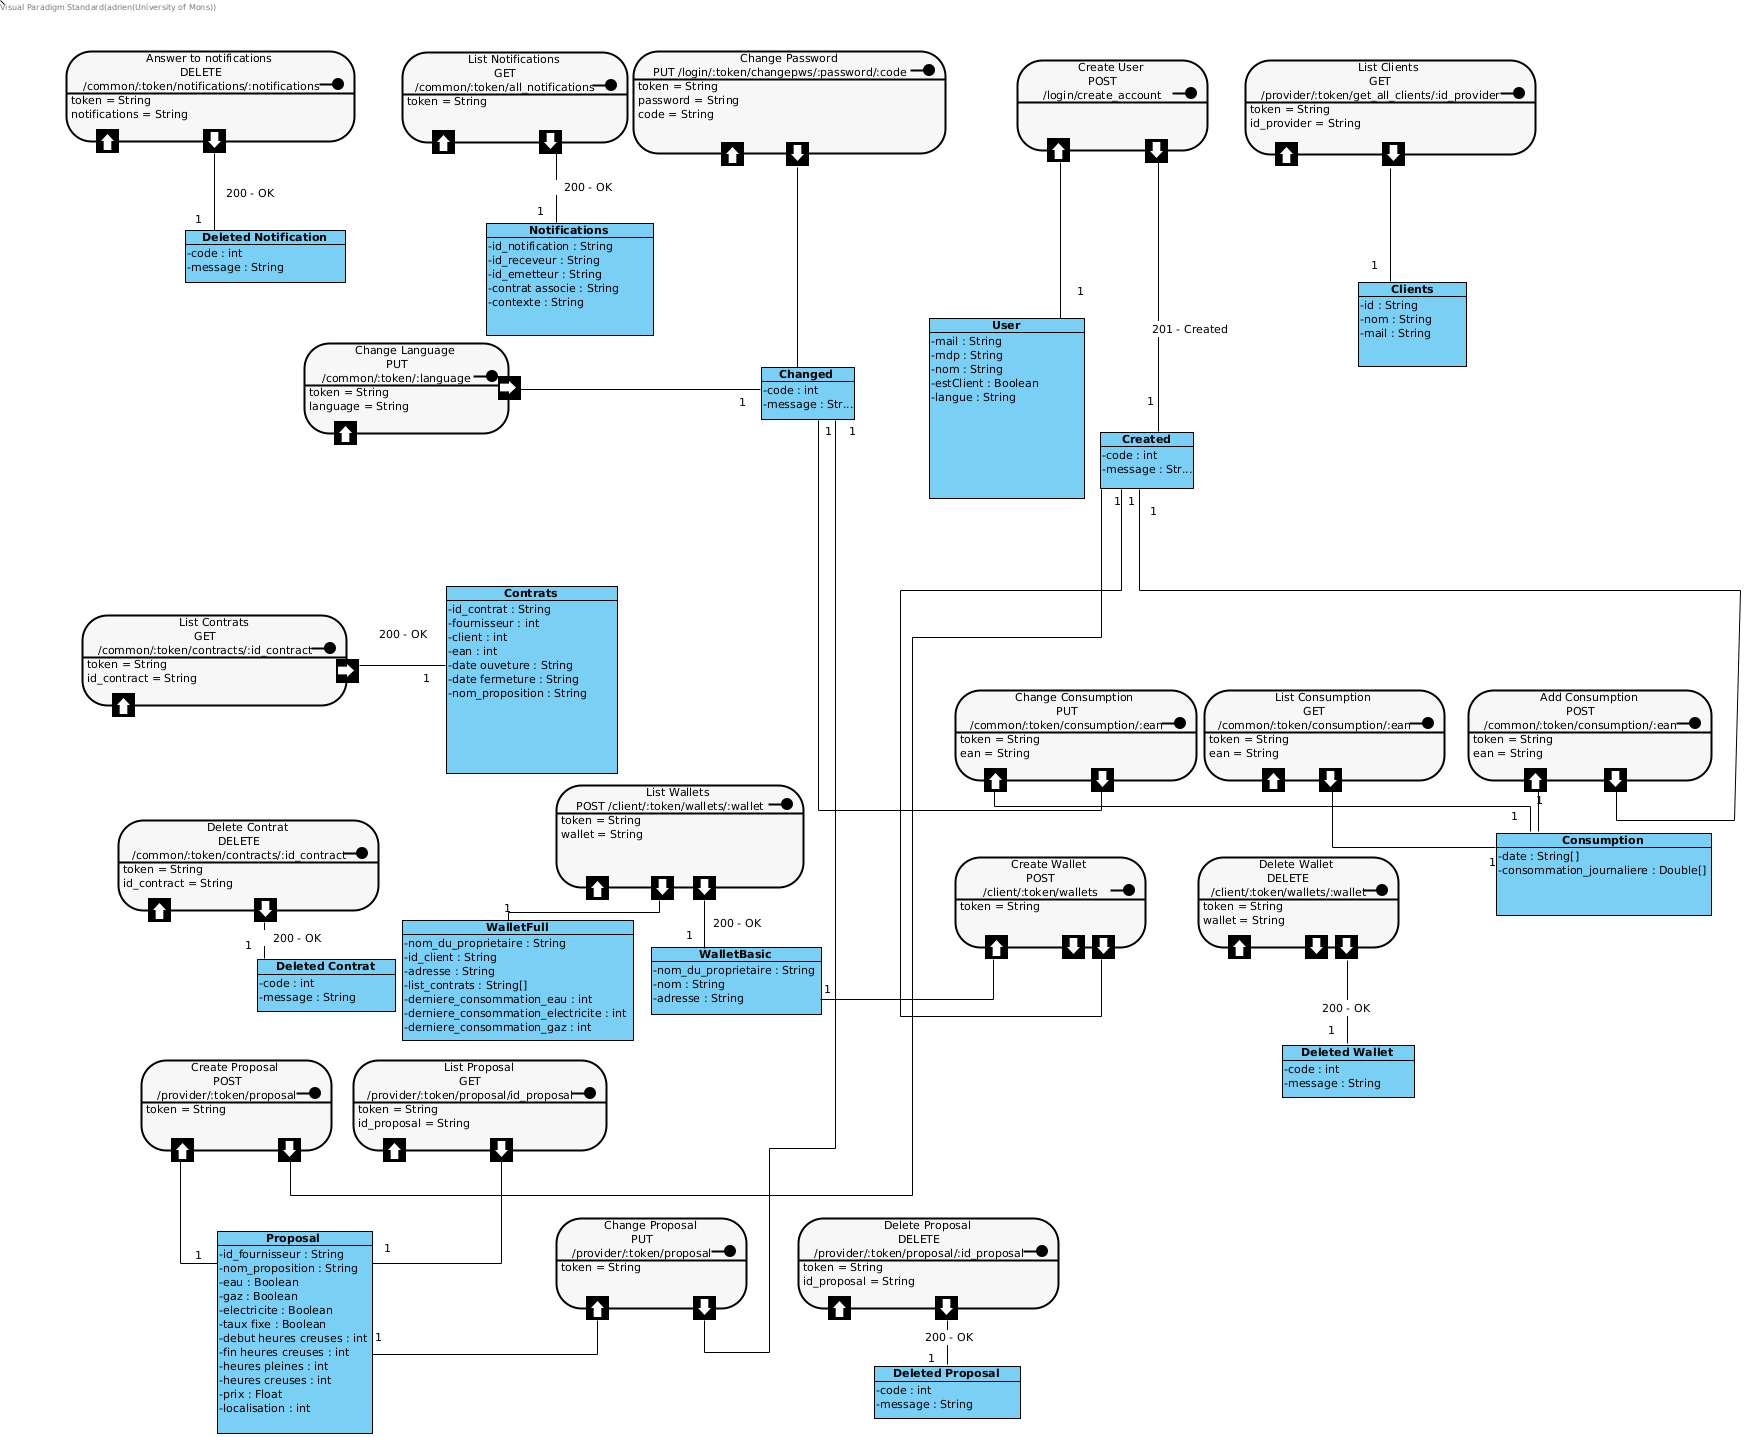
\includegraphics[width = 1.3\textwidth]{Base/api-rest/img/apirest.png}
\end{figure}

